\documentclass[]{article}

\usepackage[italian]{babel}
\usepackage[utf8]{inputenc}

\usepackage{url}
\usepackage{pdflscape}
\usepackage{booktabs}
\usepackage{float}
\usepackage{multicol}
\usepackage{lipsum}
\usepackage{graphicx}
\usepackage{caption}
\usepackage{subcaption}
\usepackage{blindtext}
\usepackage{multirow}
\usepackage[margin=1in]{geometry}
\setlength{\columnsep}{0.9cm}
%\setlength{\columnseprule}{0.5pt}

%opening
\title{La misura della Disuguaglianza nel mondo\\
	   basata sul Commercio Internazionale}
\author{Maxim Gaina, Bartolomeo Lombardi}

\begin{document}
	\maketitle
	
	\begin{abstract}
		In un mondo in cui lo sviluppo tecnologico è in grado di assumere una crescita addirittura esponenziale in certe aree, questo lavoro si basa sull'esaltazione dei sintomi di disuguaglianza a livello internazionale. Estremizzando alcuni concetti, si può dire che un gruppo di paesi esportano materie prime e lavorazioni basate su prodotti naturali a basso contenuto tecnologico, mentre un secondo gruppo, oltre a questo, basa la propria economia su esportazione ad alto valore tecnologico e servizi. Sapendo che ai beni esportati dalla prima categoria si può accedere facilmente e a basso costo, c'è una forte barriera di accesso ai beni \textit{hi-tech}, pertanto si cercherà di individuare quali sono le conseguenze per ogni partecipante del commercio internazionale, usando strumenti messi a disposizione dalla \textit{Social Network Analysis}.
	\end{abstract}
	
	\begin{multicols}{2}
	\tableofcontents
	
	\section{Non solo Pavitt}
	In economia si ritiene che la produzione, l'adozione e la diffusione di innovazioni tecnologiche siano fattori determinanti per lo sviluppo economico e cambiamento sociale, ed è per questo motivo che lo sviluppo tecnologico garantisce un alto livello del salario medio.
	
	Nel suo lavoro \cite{pavitt}, K. Pavitt cerca di evidenziare i pattern dei cambiamenti tecnologici (e quindi, dello sviluppo economico) a partire dal 1945 fino agli anni 80 nel Regno Unito. Molte tecnologie si rivelano essere \textit{informazioni} non generalmente applicabili e facilmente riproducibili, bensì \textit{specifiche} per aziende e applicazioni, \textit{cumulative} nello sviluppo, \textit{variate} tra settori sorgenti e direzioni. 
	
	Le aziende innovatrici, che operano in settori come elettronica e chimica, sono relativamente grandi e portano innovazioni su una ricca gamma di prodotti specifici, ma ne esportano poche. Le aziende specializzate in ingegneria meccanica e strumentistica sono relativamente piccole ed esistono in simbiosi con grosse aziende in settori a \textit{intensità di scala} che producono metalli di base e veicoli. D'altra parte, nelle aziende tessili le innovazioni arrivano dai fornitori. Queste variazioni vengono classificate in quattro raggruppamenti settoriali:
	\begin{enumerate}
		\item \textit{supplier dominated}, che comprende carta, legname e calzature;
		\item \textit{scale intensive}, che comprende metalli di base, autoveicoli e motori;
		\item \textit{specialized suppliers}, relativo a macchine agricole, industriali, strumenti di precisione e ottici;
		\item \textit{science based}, che riguarda i settori estremamente sensibili al progresso scientifico come chimica, farmaceutica ed elettronica.
	\end{enumerate}
	
	Nonostante il  contributo di Pavitt sia stato riconosciuto a pieni voti, è doveroso ricordare che il suo lavoro è stato pubblicato nel 1984, e che da allora il mondo sia cambiato. Infatti, non solo esistono alcune revisioni critiche verso i suoi metodi di studio \cite{archibugi}, ma possiamo anche individuare, al giorno d'oggi, almeno un'altro settore:
	\begin{enumerate}
		\item[5.] \textit{information intensive}, che riguarda la microelettronica, software e dati.
	\end{enumerate}

	Inoltre, non siamo stati in grado di trovare una classificazione precisa dei beni secondo la tassonomia di Pavitt. Un primo tentativo, quindi, è stato quello di prendere la classifica Harmonized System a due cifre\footnote{\url{http://unstats.un.org/unsd/tradekb/Knowledgebase/50043/HS-Classification-by-Section}}, e di assegnare manualmente un settore di Pavitt a ogni categoria presente nella classifica. Per esempio, la seguente categoria \texttt{HS 02: Meat and edible meat offal} avrebbe ricevuto il codice \texttt{1: Supplier dominated}. Tuttavia, ci siamo resi conto che le nostre conoscenze in commercio internazionale, non erano sufficienti per fare una classificazione manuale e che, ogni minimo errore di classificazione avrebbe portato a grandi errori nei risultati finali.
	
	\subsection{Standard International Trade Classification}
	È stata individuata una tassonomia più recente \cite{lall}, che assegna un valore a tre cifre, di \textit{intensità tecnologica}, per ogni categoria secondo lo \textit{Standard International Trade Classification Rev.2}. Questo ci ha permesso di evitare a pieno gli errori. Attualmente, lo standard SITC è alla sua versione Rev.4, ma questo non è un problema, perché confrontando la Rev.2 con la Rev.3 e Rev.4 si è visto che il numero delle categorie non aumentano o cambiano radicalmente. Le categorie a tre cifre SITC Rev.2 sono 252, mentre, le categorie che sono state classificate per intensità tecnologica nel progetto, sono 242. Le 10 categorie non menzionate sono codici speciali (come lo \texttt{031: UN Special Code}) che non hanno alcuna utilità a essere classificate. La classifica è così fatta\footnote{\url{http://unstats.un.org/unsd/tradekb/Knowledgebase/Technological-classification-of-exports-by-SITC}}:
	\begin{enumerate}
		\item prodotti non catalogati (elettricità, codici speciali, opere d'arte...);
		\item materie prime (frutta, petrolio...);
		\item lavorazioni basate su prodotti naturali (frutta preparata, olio vegetale, vetro...);
		\item prodotti \textit{low-tech} (calzature, giocattoli, semplici prodotti metallici e plasitici...);
		\item prodotti \textit{mid-tech} (veicoli e parti, acciaio, macchine industriali...);
		\item prodotti \textit{hi-tech} (macchine per processamenti dei dati, transistor, farmaci, ottica, spazio...).
	\end{enumerate}
	
	\section{Dati sotto esame}
	Questa sezione esporrà il modo in cui sono stati ottenuti i dati necessari per lo svolgimento dello studio.
	
	Nel commercio si possono scambiare non solo \textbf{beni} ma anche \textbf{servizi}. In questo lavoro, i servizi vengono ignorati, ma si può dire con certezza che anche questi sono generalmente offerti dalle economie più avanzate e che spesso riguardano il settore information-intensive. Secondo una nostra valutazione, l'introduzione dei servizi probabilmente avrebbe aumentato ancora di più il divario tra economie sviluppate e non, senza cambiare il carattere dell'esito. Tutti i dati trattati nel corso di questo progetto, cioè dati commerciali e demografici, riguardano l'anno \textbf{2015}.
	
	Prima di procedere bisogna notare il fatto che, data una transazione di beni da A verso B, A può dichiarare la transazione come export di valore $x$, mentre B dichiara la stessa transazione come import di un valore $y$. L'import ed export vengono calcolati diversamente (per esempio, l'import tiene conto anche delle spese di trasporto), ma ogni attore dichiara il valore che quel bene ha sul proprio territorio. Per esempio nel 2015, l'Italia ha esportato verso l'Afghanistan un certo numero di beni per un valore di \$8mln, ma l'Afghanistan dichiara di aver importato \$4mln dall'Italia tramite la medesima transazione. Quindi, per questo motivo, si è scelto di analizzare i dati di \textbf{import} di ogni paese.

	L'idea iniziale era quella di organizzare una rete in cui ogni nodo rappresentava un'area geografica oppure un gruppo economico regionale. La complicazione, però, consisteva nel fatto che i gruppi economici regionali si potevano sovrapporre. Infatti, uno stato può appartenere a più di un'organizzazione, ma ancor peggio è il fatto che le organizzazioni non spiegano i livelli tecnologici dei prodotti entranti per ogni membro. Esistono stati, invece, che non appartengono ad alcun gruppo. Dopo questa analisi, ci siamo soffermati sul concetto di nodo come singolo stato, e su archi orientati come direzione del flusso commerciale.
	\subsection{Preparazione dei Dati}	
	\paragraph{Raccolta dati grezzi} Sono stati raccolti dati che riguardano l'\textbf{import} di prodotti per ogni stato, raggruppato per fonte (cioè ogni altro stato fornitore), categorizzato con SITC Rev.2 del prodotto. La fonte\footnote{\url{https://comtrade.un.org/data/}} di questi dati non permette di fare query per più di 5 stati contemporaneamente e query che superano le 50.000 righe. Pertanto, sono state fatte più di 50 query per coprire tutta la lista dei paesi, escludendo i gruppi economici come l'\texttt{UE}.
	
	\paragraph{Elaborazione dei dati} I risultati delle query, in formato \texttt{.csv}, contenevano più di 30 campi per record e - stranamente - diversi tipi di ambiguità nei campi testuali che ne impedivano la corretta interpretazione. L'unione di tutte le query superavano le 1.200.000 righe, e un sottoinsieme di queste contenevano segni di punteggiatura di ogni sorta, un problema per i parser \texttt{.csv} standard. Tali difficoltà sono state superate tramite lo sviluppo di script in \texttt{Java} con l'utilizzo di espressioni regolari che hanno eliminato le ambiguità. Sono stati, quindi, scartati i campi che descrivevano la quantità dei beni scambiati e la relativa unità di misura in quanto incompleti, più altri campi che non portavano informazioni utili (per esempio, modalità di trasporto). Sono stati lasciati i seguenti campi, dove reporter è l'importatore, e partner è l'origine del prodotto:	
	\begin{center}
		\begin{verbatim}
			reportercode: 381
			reporter: Italy
			reporteriso: ITA
			
			partnercode: 704
			partner: Viet Nam
			partneriso: VNM
			
			commoditycode: 553
			tradevalue: <valore numerico, $>
		\end{verbatim}
	\end{center}

	\paragraph{Livelli tecnologici e normalizzazione} È stato necessario sapere per ogni scambio avvenuto, il relativo livello tecnologico. I livelli sono stati codificati tramite un intero $i \in [0,5]$ sotto un nuovo campo \texttt{techlevel}. In più, è stato necessario \textit{normalizzare} il valore dell'import mettendolo in rapporto con il numero degli abitanti del relativo reporter. Il risultato di questa elaborazione ha prodotto una lista di tutti gli stati con corrispettivo codice e la relativa popolazione totale. Il rapporto $\frac{tradevalue}{popolazione}$ ha dato origine al campo \texttt{importperperson}.
	\begin{center}
		\begin{verbatim}
		techlevel: 2
		importperperson: 0.0069823
		\end{verbatim}
	\end{center}
	Per ogni record, i valori di questi campi sono stati inseriti tramite appositi script sviluppati in \texttt{Java}.
	
	\paragraph{Raggruppamento degli scambi} Essendo in possesso di tutte le informazioni necessarie, ecco quanto è stato fatto:
	\begin{enumerate}
		\item query \texttt{SQL} sull'intero dataset per raggruppare gli scambi in base a \texttt{<reporter, partner, techlevel, normalizedimport>}, dove \texttt{normalizedimport} è la somma di tutti gli \texttt{importperperson};
		\item query per eliminare i record con \texttt{partner=WLD World}, evitando così un nodo con archi uscenti verso tutti, così come per eliminare record che denotano l'import da aree generiche come \texttt{ESH: Western Sahara, ATA: Antarctica} e \texttt{ATF: Fr. South Antarctic};
		\item query per eliminare i record di paesi che importano da se stessi, sarà infatti necessaria una matrice con diagonale nulla;
		\item query per estrarre e dividere le tuple in base al valore \texttt{techlevel}.
	\end{enumerate}
	Così facendo sono stati ottenuti 6 dataset, uno per ogni categoria tecnologica.
	
	\paragraph{Trasformazione in matrici} Per poter usare la funzione \textit{Tabella Pivot}, presente in \texttt{Excel}, e ottenere una matrice quadrata con diagonale nulla, evitando così l'uso di altri script, era necessario che la cardinalità degli importatori e dei partner fosse la stessa, ma ciò non accadeva. Per ogni dataset, dei sei ottenuti, accadeva che il numero dei partner distinti fosse diverso (maggiore) da quello dei reporter distinti. Quindi, attraverso query è stata ricavata la differenza insiemistica fra le due categorie e sono stati quindi inseriti dei record \textit{falsi}, senza alcun valore di scambio, per far sì che il numero degli importatori distinti uguagliasse quello dei partner.
	
	In seguito a queste trasformazioni, sono state ottenute 6 matrici di adiacenza a diagonale nulla che sono andate a formare una \textbf{multiplex}, dove i codici degli importatori sono sulle label delle colonne e assumono il ruolo di variabili, e i codici dei partner sono sulle label di riga e esprimono i casi. Le celle contengono il valore di scambio normalizzato, se è avvenuto, oppure 0. È stata così ottenuta una rete di 225 attori, costituita da legami orientati che esprimono il flusso commerciale da e verso un nodo.
	
	\subsection{Attributi dei Nodi}
	Ogni nodo ha delle proprietà che verranno descritte di seguito.
	\begin{table}[H]
		\centering
		\caption{Codifica dei continenti}
		\label{continent}
		\begin{tabular}{@{}lllll@{}}
			\toprule
			Codice & Nome & Attributo \\ \midrule
			AF & Africa & 1 \\
			AS & Asia & 2 \\
			OC & Oceania & 3 \\
			EU & Europa & 4 \\
			NA & Nord America & 5 \\
			SA & Sud America & 6 \\  \bottomrule
			\hline 
		\end{tabular}
	\end{table}
	\paragraph{Continente} Durante l'analisi, è stato utile raggruppare i nodi in base al continente. Ogni nodo presente nei dati appartiene a uno dei 6 continenti presenti nella Tabella \ref{continent}.
	\paragraph{Coordinate Geografiche}
	Allo scopo di posizionare graficamente i nodi per creare una mappa geografica, sono state inserite le longitudini e le latitudini\footnote{\url{https://developers.google.com/public-data/docs/canonical/countries_csv}} di ogni stato nel dataset. Le coordinate disponibili per gli stati sono formate da due identificativi \texttt{ALPHA}, mentre, i dati usano codici a tre. In questo modo, è stato fatto un \texttt{join} tra dati, conoscendo le corrispondenze fra codici.
	\paragraph{Human Development Index} Per comprendere meglio da un punto di vista grafico le proprietà dei nodi, è stato utile l'inserimento di una variabile che indica la qualità della vita, utilizzata poi  per effettuare analisi statistiche. Lo \texttt{HDI}\footnote{\url{http://hdr.undp.org/en/data}} è un double compreso fra 0 e 1 (più l'indice si avvicina a 1 e più le condizioni per lo sviluppo umano sono favorevoli in quel paese). L'indice tiene conto di un'altro insieme di indici: aspettativa per la vita, livello di istruzione e indice \texttt{GNI}. È stata inserita la stessa variabile ma in forma ordinale, nel caso si rivelasse più comoda, fissando i range come specificato nella Tabella \ref{hdicutoff}, dal rapporto ufficiale dell'ONU (tranne \textit{Non disponibile}).
	\begin{figure*}[b]
		\centering
		\begin{subfigure}[b]{.496\textwidth}
			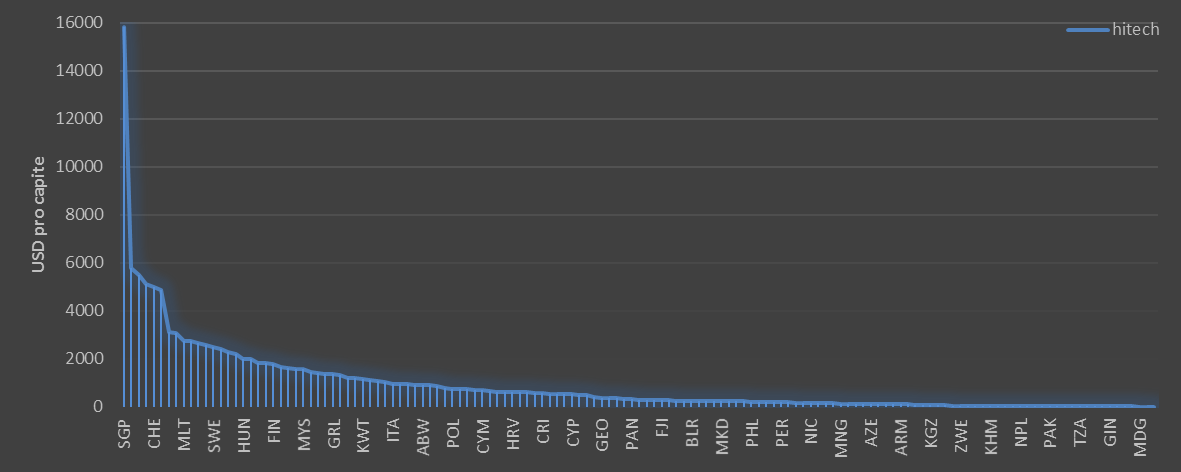
\includegraphics[width=\textwidth]{img/hitech-serie.png}
			\caption{Beni hitech}
		\end{subfigure}
		\begin{subfigure}[b]{.496\textwidth}
			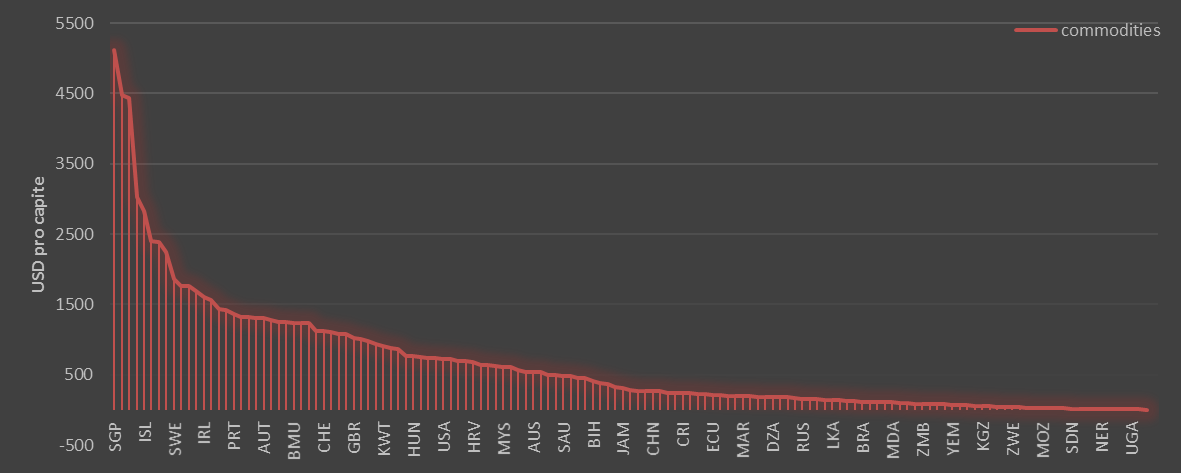
\includegraphics[width=\textwidth]{img/com-serie.png}
			\caption{Materie prime}
		\end{subfigure}
		%		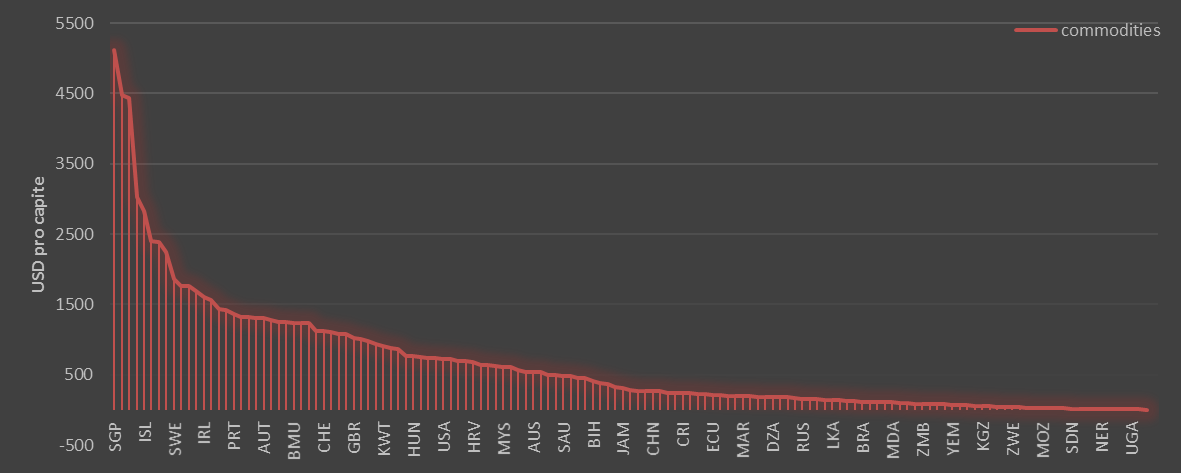
\includegraphics[scale=.82]{img/com-serie.png}
		\caption{Distribuzione del valore totale di import per persona espresso in USD, per ogni stato. N.B.: gli stati non sono ordinati nello stesso modo nei due grafici.}
		\label{fig:distribuzione}
	\end{figure*}
	\begin{table}[H]
		\centering
		\caption{Punti di cutoff per l'indice \texttt{HDI}}
		\label{hdicutoff}
		\begin{tabular}{@{}lllll@{}}
			\toprule
			Classe & Range & Codice \\ \midrule
			Very high HDI & $0.800–1$ & 4 \\
			High HDI & $0.700–0.799$ & 3 \\
			Medium HDI & $0.550–0.699$ & 2 \\
			Low HDI & $0.001–0.550$ & 1 \\ 
			Non disponibile & 0 & 0 \\ \bottomrule
			\hline 
		\end{tabular}
	\end{table}	
	Fra tutti i 225 nodi, per 38 non esisteva un indice \texttt{HDI} fornito dall'ONU. Poiché le statistiche dell'ONU riguardano stati sovrani, i dati commerciali a disposizione fanno in alcuni casi distinzione fra stati sovrani e territori che li compongono a statuto speciale, oppure stati indipendenti sulla carta, ma \textit{speciali} nella realtà, territori contesi o altro ancora. Ecco alcuni esempi: Hong Kong; Palestine; San Marino; Falkland Islands; Midway Islands; American Samoa e così via. Inizialmente, la scelta è stata quella di assegnare loro manualmente lo stesso indice HDI di uno stato che \textit{de facto} vi esercita poteri di qualsiasi tipo (per esempio, il Regno Unito controlla le isole Falkland, oppure il caso del regolamentato potere cinese su Hong Kong). In un secondo momento, tuttavia, è stato appurato che l'assegnamento forzato di un indice HDI a questi territori introduceva errori nella correlazione con subnet a cui appartenevano. Per esempio, abitare sulle isole Falkland non significa godere della stessa qualità di vita degli inglesi. In assenza di questi dati, quindi, la scelta finale per i 38 nodi in questione è stata quella di codificarli con 0 e trattarli come territori con qualità di vita da studiare a parte.
	
	\section{Analisi Rete degli Scambi}
	\subsection{Distribuzione del valore degli scambi}
	In un mondo ideale in cui tutti sono felici, definito da un'economia globale equa che riesce a integrare la totalità dei membri, per ogni livello tecnologico uno stato importa prodotti per una quantità che si discosta dalla media globale secondo un errore \textit{casuale}.
	
	Come è possibile osservare nella Fig. \ref{fig:distribuzione}, non si tratta neanche lontanamente di una distribuzione normale. Per ogni livello tecnologico, la situazione è descritta da un sottoinsieme di paesi attraversati da un enorme flusso commerciale con i restanti paesi che si scambiano briciole. Questo flusso mantiene la distribuzione \textit{a coda} per ogni livello, particolarmente ripida per prodotti \textit{hitech} e un pò meno per i beni a intensità tecnologica minore.
	\begin{figure*}[]
		\centering
		\begin{subfigure}[b]{1\textwidth}
			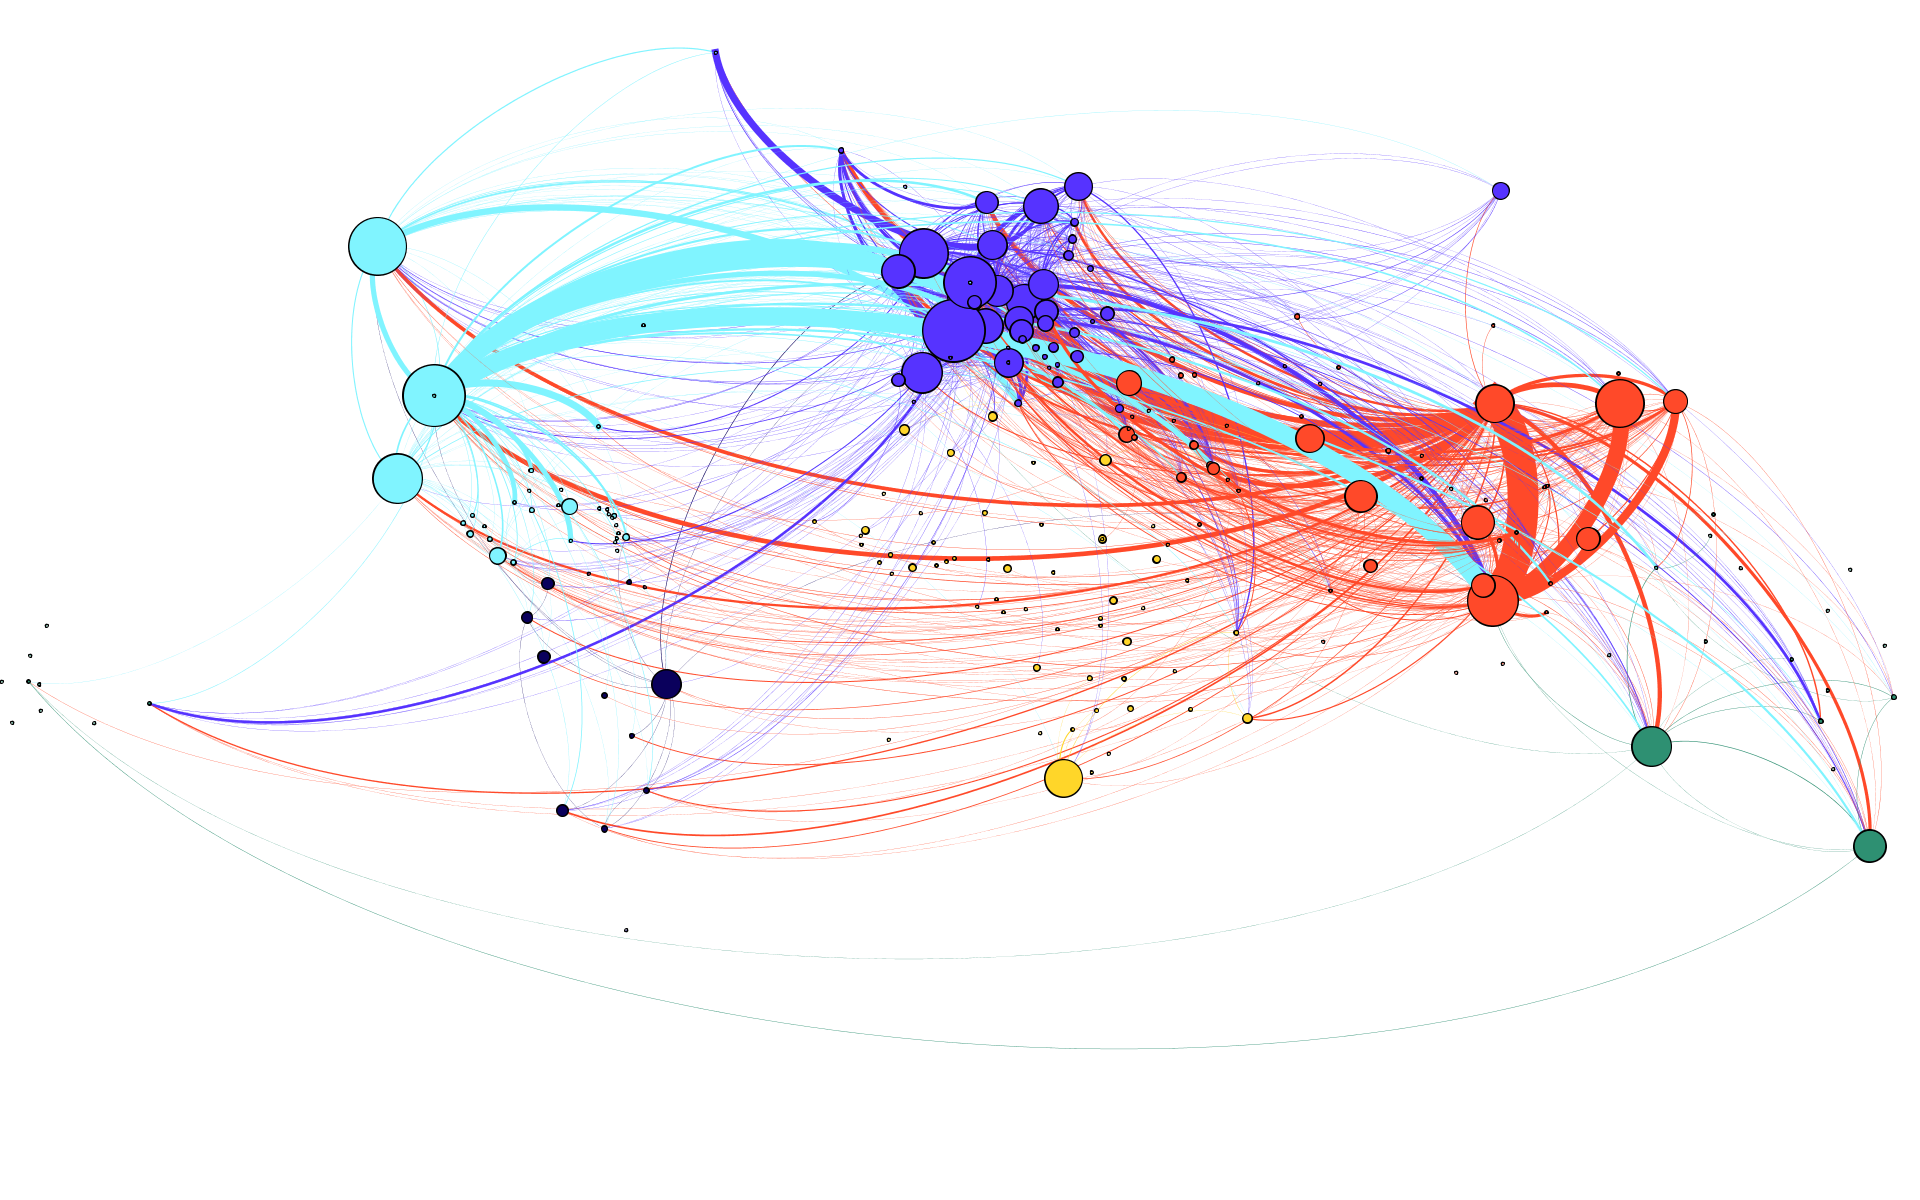
\includegraphics[width=\textwidth]{img/world-hitech.png}
			\caption{Flusso di prodotti hitech nel mondo con Cutoff dalla Tabella \ref{tab:cutoff}}
			\label{subfig:world-hitech}
		\end{subfigure}
		\begin{subfigure}[b]{1\textwidth}
			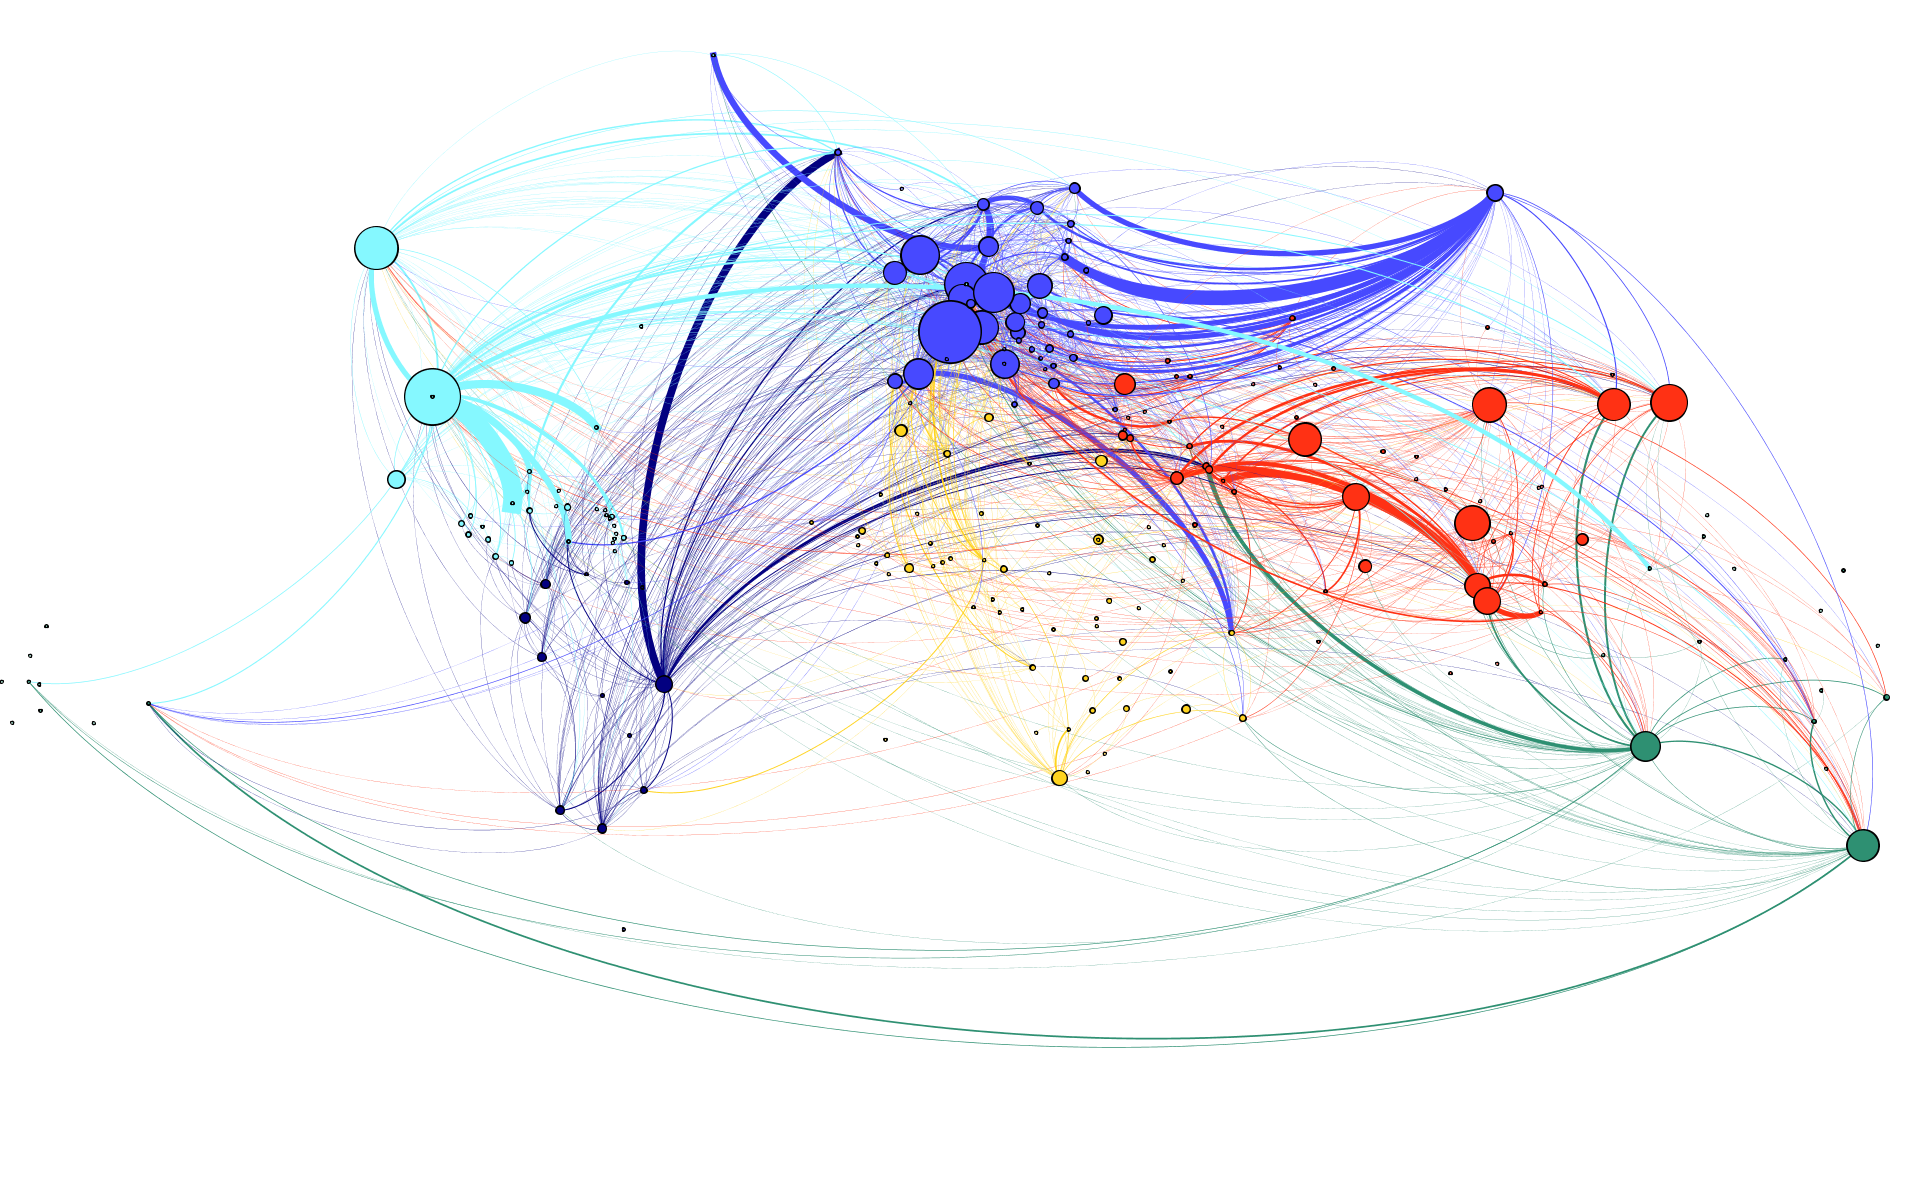
\includegraphics[width=\textwidth]{img/world-comm.png}
			\caption{Flusso di materie prime nel mondo con Cutoff dalla Tabella \ref{tab:cutoff}}
			\label{subfig:world-comm}
		\end{subfigure}
		\caption{Reti geografiche di import con spessore degli archi proporzionali al peso e colori ereditati dall'esportatore; colore del nodo in base al continente e grandezza proporzionale alla Betweennes di Freeman.}
		\label{fig:world}
	\end{figure*}
	Osservando gli scambi uno ad uno e non l'import nella sua totalità, è facile notare come gran parte delle dichiarazioni di import hanno un valore prossimo allo zero. Questo vuol dire che, numerosi posti al mondo ottengono beni per un valore normalizzato per persona, che è inferiore al singolo centesimo di dollaro. Quanto detto, viene espresso piuttosto chiaramente anche dalla Tabella \ref{tab:cutoff} dei punti di Cutoff.
	\begin{table}[H]
		\centering
		\caption{Punti di Cutoff per Livello Tecnologico}
		\label{tab:cutoff}
		\begin{tabular}{@{}lllll@{}}
			\toprule
			Livello & Scambi & Valore espresso \\ \midrule
			hitech & 8,8\% & 93,50\% \\
			midtech & 10,3\% & 93,74\% \\
			lowtech & 10,2\% & 93,71\% \\
			natural & 10,4\% & 92,30\% \\
			commodities & 11,0\% & 91,00\% \\ \bottomrule
			\hline 
		\end{tabular}
	\end{table}
	Detto in altri termini, gran parte degli archi hanno un peso bassissimo. Nella figura \ref{subfig:world-hitech}, si può vedere la minima parte più significativa degli import altamente tecnologici, e nella \ref{subfig:world-comm} gli scambi più importanti di materie prime. Si ricorda che esistono livelli intermedi di intensità tecnologica, nonostante siano visualizzati solo questi, ma una cosa risulta già chiara: \textbf{i paesi più sviluppati tendono ad avere una consistente betweenness a ogni livello tecnologico}. In Economia, è risaputo che i paesi più avanzati basano le loro attività commerciali sulla \textit{diversificazione}. Gli Stati Uniti, per esempio, non hanno bisogno di presentazioni se si parla di flusso tecnologico, ma sono anche grandi importatori di petrolio e importanti esportatori di Shale Gas (oltre che di democrazia).

	\subsection{Profilazione degli Stati}
	Data l'ipotesi iniziale, ancora da dimostrare, che il benessere è correlato al movimento dei beni altamente tecnologici, vogliamo in qualche modo individuare queste \textit{barriere hitech} che dovrebbero incidere sulla qualità della vita. Per individuarle, verrà presa in considerazione esclusivamente la rete degli scambi di prodotti \texttt{hitech}. Altri tentativi di classificazione sono stati scartati in quanto non sembravano promettenti, come ad esempio la classificazione dei nodi in una rete degli scambi a livelli sovrapposti.
	
	\paragraph*{Dicotomizzazione} Una volta isolato il livello tecnologico più alto, la classificazione su una rete ad archi pesati, dove il peso è distribuito come descritto nella sottosezione precedente, non offre grandi risultati. Il carattere della distribuzione dei pesi richiede un Cutoff per ottenere dei cluster soddisfacenti, ma proprio il Cutoff porterebbe via dal quadro paesi che è nel nostro interesse classificare. La matrice \texttt{hitech} è stata, quindi, dicotomizzata ottenendo \texttt{hitech-bin}, sostituendo 1 a ogni valore maggiore di 0, perché non era importante ragionare sui pesi.
	
	\paragraph*{Equivalenza Strutturale} E' più opportuno ragionare in termini di \textit{Equivalenza Strutturale}. Ovvero, l'ipotesi è che gli stati che fanno parte del \textit{club tecnologico} tendono a essere connessi ad altri più o meno nello stesso modo: hanno presumibilmente un buon numero di archi in entrata e in uscita. Ricordiamo che, anche nella rete \texttt{hitech}, gli importatori sono meno degli esportatori. Siamo, dunque, in presenza di un buon numero di stati - a una prima occhiata poveri - che hanno pochi archi uscenti. Ciò è probabilmente dovuto ad aziende che sfruttano la manodopera a basso costo e rimpatriano i prodotti una volta finiti. Quindi, l'ipotesi che riguarda l'equivalenza strutturale degli stati in basso alla classifica è dovuta al fatto che qualcosa lo esportino (quindi hanno qualche arco uscente), e sicuramente che qualcosa lo riescano a comprare (quindi al massimo qualche arco entrante).
	
	\paragraph*{Simmetrizzazione} Secondo alcune valutazioni empiriche, i risultati sono più soddisfacenti se viene cambiata visione: non si interpreta più la rete come un insieme di scambi direzionali, bensì come \textit{flusso} tecnologico fra due stati, quindi, ciò che considereremo importante per un pò sarà il collegamento fra due stati e non la direzione. La matrice \texttt{hitech-bin} è stata simmetrizzata in \texttt{hitech-bin-simm}.

	\paragraph*{Similarità} Il profilo di similarità di ogni nodo si è basato su \textit{distanze geodetiche}, in quanto le distanze geodetiche verso altri, dei nodi più attivi, si presume siano minori. Una volta calcolate le geodetiche fra ogni coppia di nodi, è stata usata la distanza Euclidea come misura di similarità, ignorando i valori sulla diagonale. \texttt{Ucinet} ci ha permesso, quindi, di avere il partizionamento dei nodi in base proprio al loro profilo di similarità. Per verificare in maniera intuitiva il senso dei risultati, i nodi sono stati raggruppati per cluster e colorati in base all'indice \texttt{HDI}. Nella figura \ref{fig:profiles}, si può osservare il raggruppamento migliore da noi ottenuto. Tale raggruppamento, in realtà, presenta anche un piccolo ritocco manuale. Infatti, i cluster erano 6, di cui 4 erano esattamente come nella figura \ref{fig:profiles}, mentre, i restanti 2 cluster erano composti ciascuno da un unico nodo. Per evitare di avere, in un secondo momento, una matrice a blocchi con una riga considerata come blocco, questi nodi sono stati spostati nei cluster, ai quali appartenevano nei precedenti passi di clustering, dove però la suddivisione degli altri nodi non era così qualitativa. 
	\begin{figure*}[t]
		\centering
		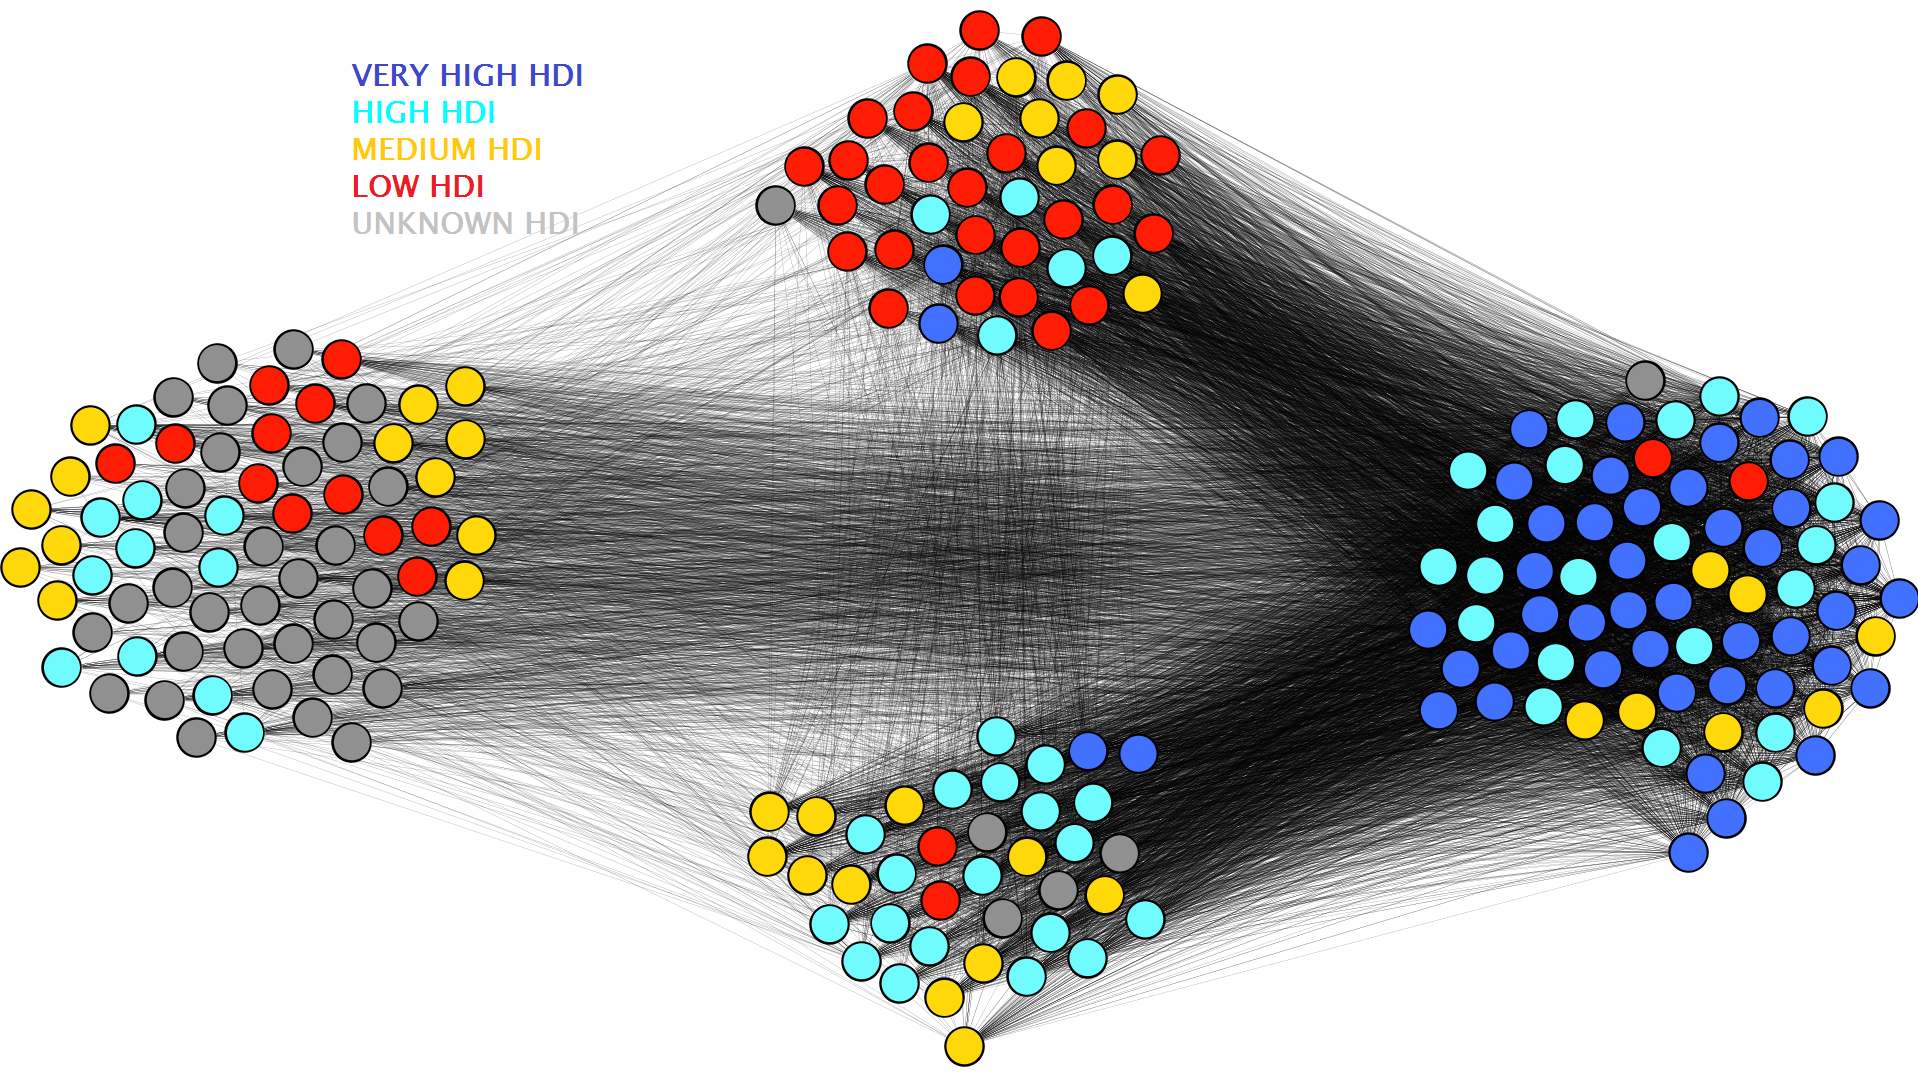
\includegraphics[scale=.4]{img/profiles.png}
		\caption{Stati raggruppati secondo clustering su distanze geodetiche, colorati in base alla classe \texttt{HDI}}
		\label{fig:profiles}
	\end{figure*}
	Ecco alcune osservazioni:
	\begin{enumerate}
		\item il cluster più a destra è dominato dagli stati con indice \texttt{HDI} alto e molto alto, c'è qualche eccezione come il Pakistan che, pur essendo un paese con l'indice \texttt{HDI} basso è più connesso agli altri rispetto quelli della sua stessa categoria, questo perché viene usato per la forza lavoro;
		\item il cluster più in alto è dominato dagli stati con indice \texttt{HDI} basso, ad eccezione dei due nodi: Brunei e Kuwait;
		\item il cluster più a sinistra è lievemente più eterogeneo, ma si può notare come la maggior parte dei territori senza un indice \texttt{HDI} si trovino proprio qui, mentre le aspettative erano che fossero sparsi ovunque;
		\item quello in basso rappresenta \textit{l'angolo dei mediocri}, il cluster è conteso dai nodi con indice medio e alto.
	\end{enumerate}
	È stata data un'interpretazione del risultato, ma servirebbe un feedback statistico del fatto che il raggruppamento sia sensato, facendo riferimento alla Tavola di Contingenza della Tabella \ref{tab:contingenza}. Per ogni cluster, il metodo fin'ora presentato riesce ad individuare una maggioranza di classe \texttt{HDI}, e riesce, per le due classi \texttt{HDI} all'estremità (0, 1 e 4), a mettere la maggior parte dei nodi che le compongono nello stesso cluster. Mentre, le classi 2 e 3 sono quelle più sparse avendo un profilo più \textit{nel mezzo}.	
	\begin{table}[H]
		\centering
		\caption{Tavola di Contingenza, variabile nominale Cluster sulle colonne e ordinale HDI Class su righe; per ogni cella sopra la percentuale entro \texttt{Classe}, sotto la percentuale entro \texttt{Cluster}.}
		\label{tab:contingenza}
		\begin{tabular}{@{}ccccc@{}}
			\toprule
			\multicolumn{1}{l}{} & \begin{tabular}[c]{@{}c@{}}CL221\\ Ignorati\end{tabular} & \begin{tabular}[c]{@{}c@{}}CL225\\ Poveri\end{tabular} & \begin{tabular}[c]{@{}c@{}}CL222\\ Medi\end{tabular} & \begin{tabular}[c]{@{}c@{}}CL223\\ Ricchi\end{tabular} \\ \midrule
			\multirow{2}{*}{HDI 0} & \textbf{85,00\%} & 2,50\% & 10,00\% & 2,50\% \\
			& \textbf{48,60\%} & 2,30\% & 10,50\% & 1,40\% \\ \midrule
			\multirow{2}{*}{HDI 1} & 27,90\% & \textbf{62,80\%} & 4,70\% & 4,70\% \\
			& 17,10\% & \textbf{62,80\%} & 5,30\% & 2,70\% \\ \midrule
			\multirow{2}{*}{HDI 2} & 33,30\% & 20,50\% & 28,20\% & 17,90\% \\
			& 18,60\% & 18,60\% & 28,90\% & 9,50\% \\ \midrule
			\multirow{2}{*}{HDI 3} & 19,60\% & 8,90\% & \textbf{33,90\%} & 37,50\% \\
			& 15,70\% & 11,60\% & \textbf{50,00\%} & 28,40\% \\ \midrule
			\multirow{2}{*}{HDI 4} & 0,00\% & 4,30\% & 4,30\% & \textbf{91,50\%} \\
			& 0,00\% & 4,70\% & 5,30\% & \textbf{58,10\%} \\ \bottomrule
		\end{tabular}
	\end{table}
	Interpretando \texttt{Cluster} come variabile nominale indipendente e \texttt{Class} come intervallo discreto dipendente, otteniamo che il relativo coefficiente direzionale \texttt{Eta} è dello $0,707$ il che suggerisce che c'è \textbf{una buona correlazione fra le due variabili}. Sostituendo, invece, \texttt{Class} con il vero indice \texttt{HDI}, che è un intervallo continuo fra $0$ e $1$, il coefficiente \texttt{Eta} ricavato nello stesso modo risulta $0,681$. Pertanto, si può dire che, più uno stato scambia beni tecnologici con un maggior numero di attori, più tende a essere benestante.
	
	\subsection{Rapporto fra Gruppi di Stati}
	Ci si aspetta che quanto appena detto non valga \textit{così fortemente} se scendiamo di livello tecnologico. Infatti, probabilmente la densità e il valore degli scambi continueranno a essere più alti tra paesi benestanti a causa del principio di \textit{diversificazione}, ma ci si aspetta, allo stesso tempo, che i confini non siano così netti per le materie prime. In totale, nel 2015 sono stati registrati $16.121$ scambi \texttt{hitech} fra i nodi in esame. Come si può vedere nella Tabella \ref{tab:scambi-cluster}, quasi un terzo degli scambi avviene nel Cluster 4, quello dei ricchi.
	\begin{table}[H]
		\centering
		\caption{Numero degli scambi fra gruppi di stati}
		\label{tab:scambi-cluster}
		\begin{tabular}{@{}lcccc@{}}
			\toprule
			& \multicolumn{1}{l}{CL1} & \multicolumn{1}{l}{CL2} & \multicolumn{1}{l}{CL3} & \multicolumn{1}{l}{CL4} \\ \midrule
			CL1 & 15                      & 205                     & 220                     & 1711                    \\
			CL2 & 22                      & 596                     & 251                     & 1919                    \\
			CL3 & 23                      & 213                     & 308                     & 1700                    \\
			CL4 & 208                     & 1688                    & 2803                    & \textbf{4958}                    \\ \bottomrule
		\end{tabular}
	\end{table}
	Le densità sono calcolate sulla rete dicotomizzata \texttt{hitech-bin}. Se invece viene ricavata la densità basata sui pesi della rete \texttt{hitech}, si vede come, non un terzo, ma quasi la maggior parte del valore degli scambi, viene trattenuto nel Cluster 4. Questo si intuiva all'inizio, parlando di distribuzione del valore degli scambi, e lo si vede nella Tabella \ref{tab:scambi-valore-cluster}.
	\begin{table}[H]
		\centering
		\caption{Per ogni cella, sopra la somma dei valori scambiati, sotto la media dei loro valori}
		\label{tab:scambi-valore-cluster}
		\begin{tabular}{@{}lrrrr@{}}
			\toprule
			& \multicolumn{1}{c}{CL1} & \multicolumn{1}{c}{CL2} & \multicolumn{1}{c}{CL3} & \multicolumn{1}{c}{CL4} \\ \midrule
			\multirow{2}{*}{CL1} & 58,0                    & 6,2                     & 18,6                    & 26,6                    \\
			& 0,012                   & 0,002                   & 0,007                   & 0,005                   \\ \midrule
			\multirow{2}{*}{CL2} & 9,1                     & 86,2                    & 21,9                    & 70,7                    \\
			& 0,003                   & 0,048                   & 0,013                   & 0,022                   \\ \midrule
			\multirow{2}{*}{CL3} & 120,0                   & 71,9                    & 158,1                   & 164,3                   \\
			& 0,045                   & 0,044                   & 0,112                   & 0,058                   \\ \midrule
			\multirow{2}{*}{CL4} & 3705,1                  & 5037,8                  & 9742,8                  & \textbf{107624,4}       \\
			& 0,715                   & 1,583                   & 3,465                   & \textbf{19,923}         \\ \bottomrule
		\end{tabular}
	\end{table}
	Le densità sono state calcolate per tutte le altre reti: \texttt{midtech}; \texttt{lowtech}; \texttt{natural} e \texttt{commodities}.
	
	\subsubsection{Scambi interni}
	Prelevando la diagonale della matrice di densità basata sulle somme dei pesi per ogni livello, e trasformando queste diagonali in colonne, risulta una tabella livello per cluster che esprime lo \textbf{scambio interno}. Come si può vedere nella Figura \ref{subfig:scambi-cluster123}, i cluster fuori dal circolo tecnologico basano i loro scambi interni su lavorazioni a base di risorse naturali, eccetto la categoria degli ignoti che mostra qualche segno di vita per quanto riguarda il contenuto tecnologico di medio livello. E' evidente che, l'intensità tecnologica è inversamente proporzionale al valore totale degli scambi, eccetto le risorse, che i paesi con basso \texttt{HDI} spesso possiedono. Il cluster dei benestanti è stato isolato nella Figura \ref{subfig:scambi-cluster4}, in quanto, assolutamente fuori scala e fuori rapporto rispetto ad altri. Infatti, si può notare come gli scambi si basano per la maggiore sul contenuto tecnologico medio e muovono beni altamente tecnologici tanto quanto consumano lavorazioni su risorse naturali.
	\begin{figure*}[t]
		\centering
		\begin{subfigure}[b]{1\textwidth}
			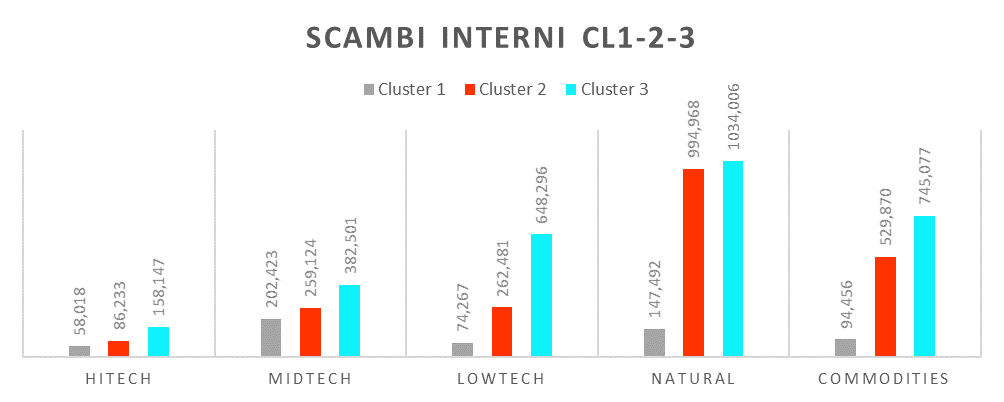
\includegraphics[width=\textwidth]{img/scambi-cluster123.png}
			\caption{Valore degli scambi interni ai cluster 1, 2 e 3 raggruppati per livello tecnologico.}
			\label{subfig:scambi-cluster123}
		\end{subfigure}
		\begin{subfigure}[b]{1\textwidth}
			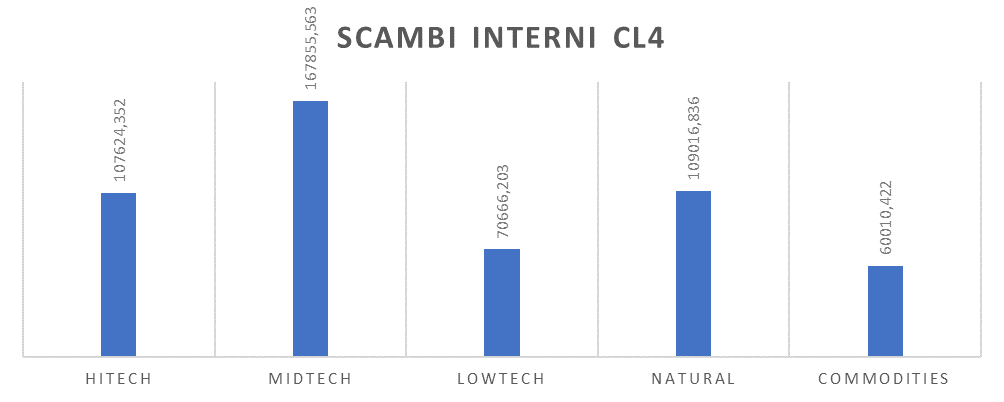
\includegraphics[width=\textwidth]{img/scambi-cluster4.png}
			\caption{Valore degli scambi interni al cluster 4 raggruppati per livello tecnologico.}
			\label{subfig:scambi-cluster4}
		\end{subfigure}
		\caption{Caratteristiche degli scambi interni ai cluster individuati}
		\label{fig:scambi}
	\end{figure*}

	\subsubsection{Scambi esterni}
	Per capire la natura dei rapporti esterni fra il quarto cluster e gli altri, è stata esaminata la riga e la colonna $4$ per ognuna delle $5$ matrici di densità. La quarta riga rappresenta il flusso uscente dal circolo dei benestanti, mentre, la quarta colonna rappresenta le entrate provenienti dagli altri gruppi. Nella Figura \ref{fig:import-cl4}, si può vedere quanti \texttt{USD} pro capite importa il Cluster 4 dagli altri. È evidente che, il fabbisogno dei paesi avanzati sale in maniera inversamente proporzionale all'intensità tecnologica, ciò perché i produttori di manufatti tecnologici sono loro stessi. 
	\begin{figure*}[th!]
		\centering
		\begin{subfigure}[b]{0.75\textwidth}
			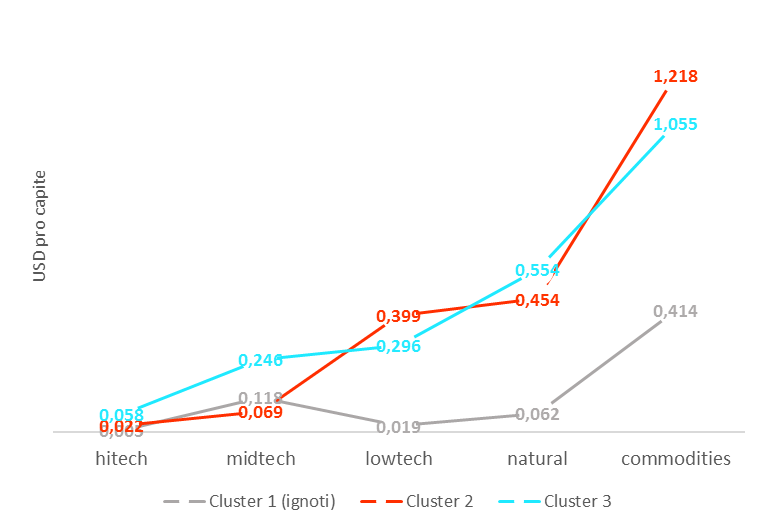
\includegraphics[width=\textwidth]{img/cl4-import.png}
			\caption{Import CL4 raggruppati per livello tecnologico}
			\label{fig:import-cl4}
		\end{subfigure}
		\begin{subfigure}[b]{0.75\textwidth}
			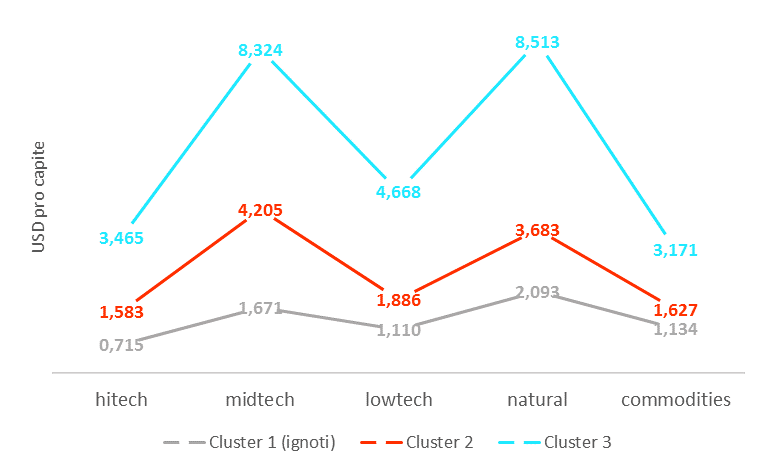
\includegraphics[width=\textwidth]{img/cl4-export.png}
			\caption{Export CL4 raggruppati per livello tecnologico}
			\label{fig:export-cl4}
		\end{subfigure}
		\caption{Relazioni esterni con altri cluster dal punto di vista del Cluster 4, dei benestanti.}
		\label{fig:import-export-cl4}
	\end{figure*}
	Nella Figura \ref{fig:export-cl4}, si nota come \textit{il resto del mondo} desidera, per la maggiore, importare beni di media intensità tecnologica e lavorazioni basate su prodotti naturali: ciò significa che necessitano di più veicoli e macchine industriali per poter progredire nell'industria, e si interessano proprio di fabbricazione di prodotti naturali.
	
	Qualcosa di proibitivo salta però all'occhio nella Figura \ref{fig:import-export-cl4}, ed è il prezzo di scambio: \textbf{i paesi avanzati dichiarano di importare prodotti di qualsiasi tipo che non superano quasi mai il dollaro per persona, quelli con indice \texttt{HDI} più basso per qualsiasi tipo di prodotto spendono abbondantemente sopra il dollaro per persona}, anche se si tratta di materie prime. Sulla rete \texttt{total}, che esprime gli scambi totali senza fare distinzione di livello tecnologico (inclusi i prodotti non classificati fin'ora ignorati), è stata creata una prima partizione che contiene i cluster 1, 2 e 3, e una seconda che contiene solo il cluster 4. Ebbene, i paesi benestanti dichiarano di importare beni per un valore medio di \$$1,459$ per persona, mentre, i restanti dichiarano di importare per un valore medio di \$$13,895$ per persona. Le barriere di accesso ai beni altamente tecnologici, così come per altri, risultano piuttosto evidenti. Tutto ciò, vale anche se consideriamo benestante il Cluster 3, confrontandolo con 1 e 2.
	
	\section{Conclusione}
	A partire da una visione di rete, l'obiettivo di questo lavoro di progetto era quello di individuare nell'insieme degli stati una serie di barriere che delimitano la parte più abbiente del pianeta e quella che lo è meno, con il presupposto che queste barriere si instaurassero in base ad aree più o meno tecnologicamente intense.
	
	Per fare ciò, in seguito alla scelta di una tassonomia più accurata possibile in base alla classificazione \texttt{SITC Rev.2}, è stata messa in atto una precisa raccolta ed elaborazione dei dati di import internazionali del 2015. Sono stati fatti lavori di pulizia a livello di nodo, lasciando in cantiere solo gli stati, talvolta non completamente sovrani, e lavori di raggruppamento a livello di archi che hanno permesso di creare una scala ordinale di intensità tecnologica degli scambi.
	
	Isolando il livello tecnologico più alto, sono poi state individuate quattro principali categorie di stati in base al profilo di similarità calcolato, riprendendo il concetto di equivalenza strutturale. Le suddivisioni, pur non essendo completamente omogenee al loro interno, spiegano piuttosto bene le aspettative per la qualità della vita misurata in base allo \textit{Human Development Index}, con un coefficiente di correlazione Eta dello $0,707$.
	
	Ecco quanto si può dire in base all'analisi della rete:
	\begin{itemize}
		\item i paesi benestanti hanno un flusso commerciale di diversi gradi più alto, a qualsiasi livello tecnologico;
		\item solo a livello \textit{hitech} i confini delle attività commerciali sono estremamente marcati, altrove il flusso commerciale riesce a scavalcare meglio tali barriere;
		\item sorprendentemente, i territori non assegnatari di un indice \texttt{HDI} da parte dell'\texttt{ONU} tendono a somigliarsi strutturalmente nella rete;
		\item il gruppo con stati non classificati, quello con prevalenza ad \texttt{HDI} basso e il terzo con prevalenza di indici \texttt{HDI} nella media, basano il loro giro d'affari interni su produzioni a base di risorse naturali, con uno scambio medio di \$$1034$ a testa (contro i \$109.016,84 a testa dei ricchi), media inversamente proporzionale all'aumentare dell'intensità tecnologica;
		\item i paesi benestanti seguono leggi diverse: hanno un giro d'affari interno basato per la maggiore sui prodotti a intensità tecnologica media, con \$$167.855,56$ a testa, al secondo posto troviamo i prodotti \textit{hitech} e le produzioni basate su risorse naturali con uno scambio medio di \$$108.000,00$ a testa, mentre al terzo posto prodotti \texttt{lowtech} e risorse con uno scambio medio nell'ordine dei \$$65.000,00$ a testa;
		\item il flusso uscente dai paesi poveri è inversamente proporzionale all'intensità tecnologica, cioè vendono molte più risorse naturali e la media di scambio più alta di \$$1,20$ a testa;
		\item il flusso entrante nei paesi poveri è dominato dal settore \texttt{midtech} e produzioni basate su risorse naturali, con media di scambio di \$$8,5$ a testa;
	\end{itemize}
	Il lavoro è stato svolto da due studenti di informatica, ma non ci vogliono competenze economiche altissime per intuire che le condizioni appena descritte sono estremamente sfavorevoli per una buona fetta di paesi.
	
	Si può affermare, quindi, con un margine di errore trascurabile e senza un'ulteriore conoscenza in materia, che uno stato più è coinvolto nello scambio di prodotti altamente tecnologici più le sue condizioni di vita sono favorevoli. Ma arrivare ad avere una centralità più alta in ambienti tecnologici non è facile, in quanto, le proprie materie di export vengono acquistate a basso costo da chi ha una posizione di potere più alta.
	
	\begin{thebibliography}{9}
		\bibitem{pavitt}
		Keith Pavitt,
		\emph{Sectoral patterns of technical change: Towards a taxonomy and a theory},
		1984.
		
		\bibitem{archibugi}
		Daniele Archibugi,
		\emph{Pavitt's Taxonomy Sixteen Years On: A Review Article},
		Economics of Innovation and New Technology 10,
		2001
		
		\bibitem{lall}
		Sanjaya Lall,
		\emph{The Technological Structure and Performance of Developing Country Manufactured Exports},
		QEH Working Paper Series,
		Working Paper Number 44,
		1998
	\end{thebibliography}
	\end{multicols}

	\begin{landscape}
		\pagenumbering{gobble}
		\begin{center}
			\begin{figure*}[th!]
				\centering
				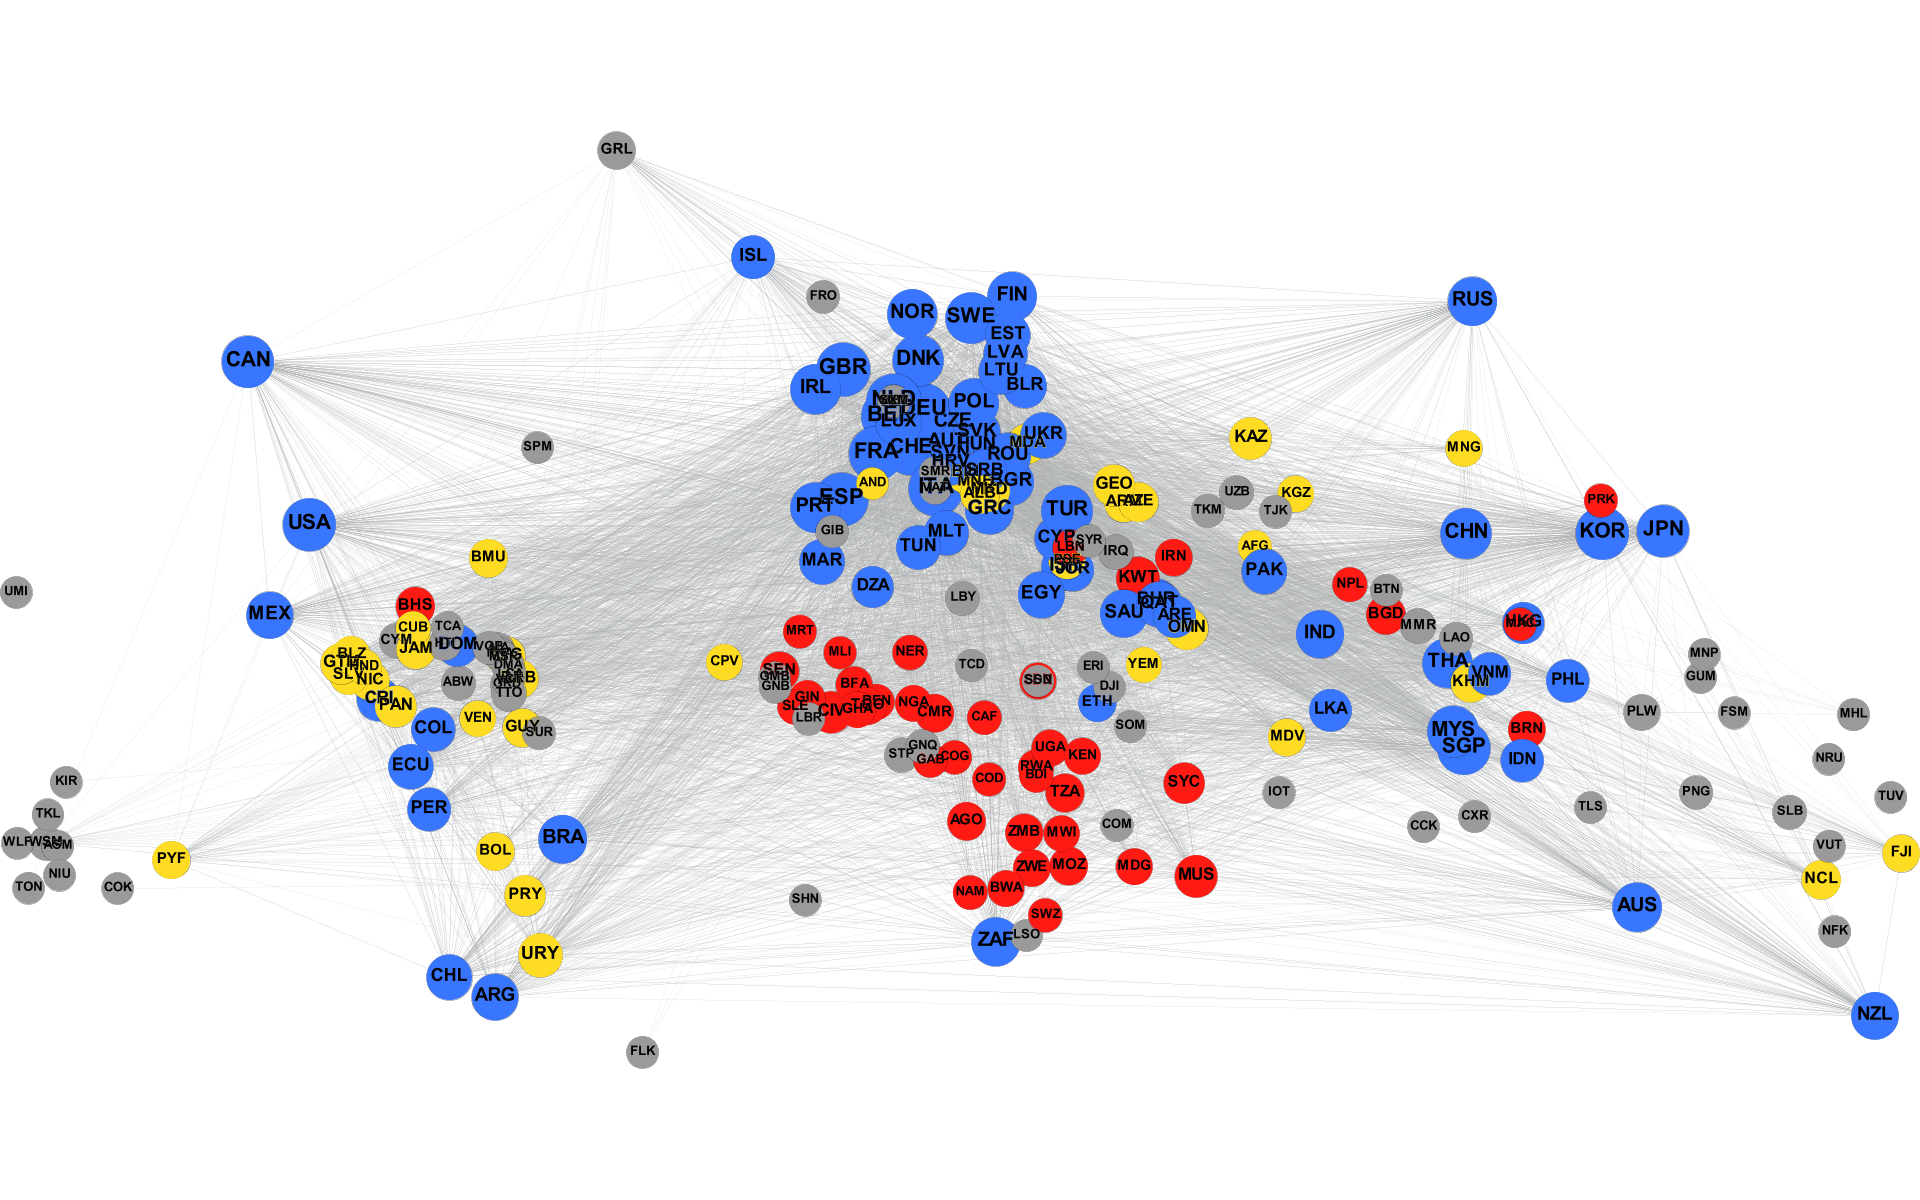
\includegraphics[scale=.35]{img/world-cluster.png}
				\caption{Visualizzazione della rete geografica colorata in base ai cluster, scambi totali con Cutoff}
				\label{fig:world-cluster}
			\end{figure*}
		\end{center}
	
		\newpage
		\begin{center}
			\begin{figure*}[th!]
				\centering
				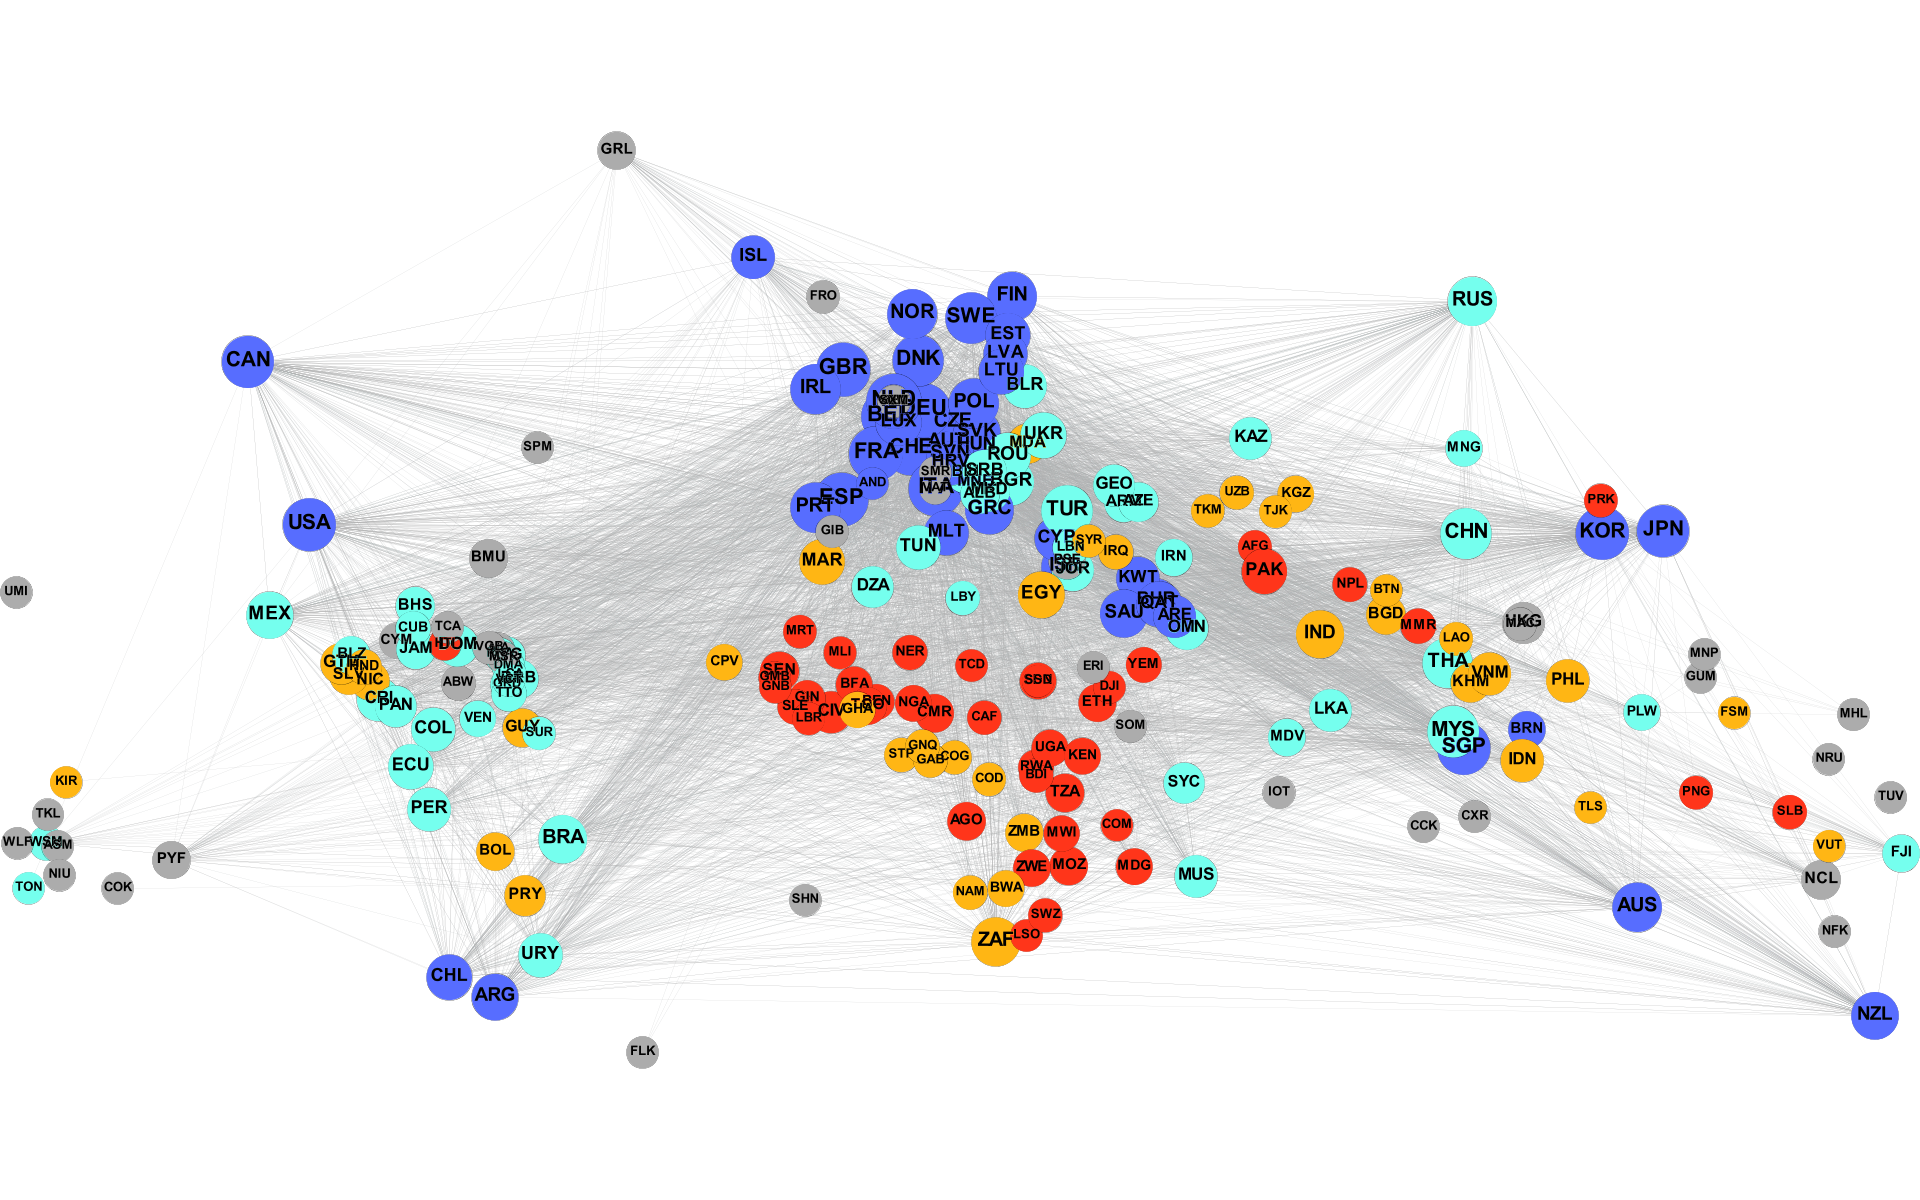
\includegraphics[scale=.35]{img/world-hdi.png}
				\caption{Visualizzazione della rete geografica colorata in base alle classi \texttt{HDI}, scambi totali con Cutoff}
				\label{fig:world-hdi}
			\end{figure*}
		\end{center}
		\end{landscape}
\end{document}
